\documentclass[t, 10pt]{beamer}
%%\documentclass[t,handout]{beamer}

\usepackage{graphicx}
\usepackage{epsfig}
\usepackage{psfrag}
\usepackage[english]{babel}
\usepackage{color}
%Mathematics packages
\usepackage{amsmath}
\usepackage{mathrsfs}
\usepackage{amsfonts}

\usepackage{enumerate}


\graphicspath{{./images/}} % Figures path - used in graphicx

\selectcolormodel{cmyk}

\mode<presentation>

%THEMES - Please refer to these chapters in the beamer documentation.
% Presentation themes : Chapter 15
% Color themes : Chapter 17
% Font themes : Chapter 18


\usetheme{Pittsburgh}
\usecolortheme{orchid}
\usefonttheme{default}

%---------------------------Title frame definition------------------------------------- 

\title{Managed Control of Composite Cloud Systems}
\author [Chris]{Christopher C. Lamb, Pramod A. Jamkhedkar, Gregory L. Heileman, and Chaouki T. Abdallah}
\institute[University of New Mexico]{
\inst {}Department of Electrical and Computer Engineering\\
University of New Mexico}
\date{June 10, 2011}
\titlegraphic{
\begin{figure} 

\includegraphics[width = 7cm]{UNM}
\end{figure}}

% Delete this, if you do not want the table of contents to pop up at
% the beginning of each subsection:
%\AtBeginSubsection[]
%{
%  \begin{frame}<beamer>
%    \frametitle{Outline}
%     \tableofcontents[currentsection,currentsubsection]
%  \end{frame}
%}

\begin{document}

\begin{frame}
\titlepage
\end{frame}

% This command will make the logo appear on all frames excluding the title frame.
\logo {
\includegraphics[width = 2.5cm]{UNM}}

\begin{frame}
\frametitle{Outline}
\tableofcontents 
\end{frame}

\section{UNM Informatics}
\begin{frame}
\frametitle{Areas of Study}

Our group:
\begin{itemize}
\item \textit{UNM Informatics}: Information security, theory, and architectures; this work is specific to information security 
\item \textit{Usage Management}: Control of how an artifact is used, covering everything \textit{after} access as well as controlling access itself
\end{itemize}
\pause

\textit{Motivation}: We believe people should have control over their own information.  Or past motivation for DRM work was to provide content control to content creators.  Doing so provides incentive for innovation, and improves quality of life for individuals and society as a whole over time.  We believe Usage Management provides the same benefits, and should be unobtrusive.
\newline
\newline
This motivation holds in this domain as well.
\pause

Acronyms:
\begin{itemize}
\item \textit{UM}: Usage Management
\item \textit{PMR}: Personal Medical Record (this is also electronic, in this case)
\end{itemize}

\end{frame}

\section{Usage Management and Cloud Systems}
\begin{frame}
\frametitle{Why is this important?}
Utility computing will certainly be the most pervasive future computing model \\
\pause
\begin{itemize}
\item \textit{Mainframes won!}
\pause
\begin{itemize}
\item Well, end devices are powerful
\item Cloud computing pervasive for \textit{convenience}, not \textit{technical necessity}.
\item \textit{Still resembles centralized models of the past}
\end{itemize}
\pause
\item \textit{People should control what they own}
\begin{itemize}
\item Access
\item Retention
\item Distribution
\end{itemize}
\pause \textit{Organizations should control what they pay for}
\begin{itemize}
\item Systems
\item Data
\item Records
\end{itemize}
\end{itemize}
\end{frame}

\begin{frame}
\frametitle{Problems}
So this is what we would like to see, but problems abound
\begin{itemize}
\item \textit{Scalability, performance, usability, infrastructural support...}
\end{itemize}
\pause

Started examining automation and ability to combine service level agreements (SLAs)
\begin{itemize}
\item \textit{Automation} \\
How we can automate control and enforcement
\item \textit{Combine} \\
How we can combine multiple SLAs into single SLAs
\end{itemize}
\pause

Surprisingly difficult...
\begin{itemize}
\item \textit{NP-Complete} \\
Simple generalized SLAs are equivalent to \textit{SAT}
\item \textit{Multiple Providers} \\
Difficult constant factors related to latency, etc.
\end{itemize}
 
\end{frame}

\section{Example Systems}
\begin{frame}
\frametitle{Single Provider, Feedback}

\end{frame}

\begin{frame}
\frametitle{Single Provider, Feedback with UM}

%\begin{figure}
%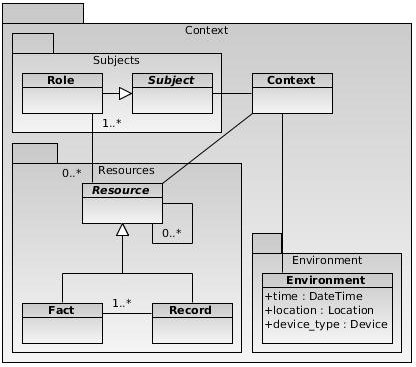
\includegraphics[width = 6cm]{UMOntology}
%\end{figure}

\end{frame}

\begin{frame}
\frametitle{Multiple Providers}

\end{frame}

\begin{frame}
\frametitle{Conclusions}

\end{frame}

%\bibliographystyle{plain}
%\bibliography{drm}

\end{document}

